% DO NOT COMPILE THIS FILE DIRECTLY!
% This is included by the other .tex files.

\begin{frame}[t,plain]
\titlepage
\end{frame}

\begin{frame}
    \frametitle{\texttt{\$ whoami}}
    \begin{center}
        
\includegraphics[width=0.3\linewidth]{pictures/whoami.png}
        \hspace{1em}
        \frame{
\includegraphics[width=0.5\linewidth]{pictures/belgian-joke}}
    \end{center}
\end{frame}

\begin{frame}
    \frametitle{Automation in MISP: What already exists?}
    
\includegraphics[valign=m,width=16px]{pictures/python-logo.png}\hspace*{0.5em} \textbf{MISP API / PyMISP}
    \hspace*{0.25em}
    \begin{itemize}
        \item Needs CRON Jobs in place
        \item Not realtime
    \end{itemize}
    \vspace*{1em}
    
\includegraphics[valign=m,width=16px]{pictures/zeromq.png}\hspace*{0.5em} \textbf{PubSub channels}
    \hspace*{0.25em}
    \begin{itemize}
        \item After the actions happen: No feedback to MISP
        \item Tougher to put in place \& to share
    \end{itemize}
    \vspace*{0.5em}
    $\rightarrow$ No way to \textbf{prevent} behavior\\
    $\rightarrow$ Difficult to setup \textbf{hooks} to execute callbacks
\end{frame}

\begin{frame}
    \frametitle{What type of use-cases are we trying to support?}
    \vspace{-1em}
    \begin{center}
        
\includegraphics[width=0.5\linewidth]{pictures/geekweek75.jpg}
    \end{center}
    \begin{itemize}
        \item \textbf{Prevent} default MISP behaviors to happen
        \begin{itemize}
            \item Prevent \textbf{publication of events} not passing sanity checks
            \item Prevent \textbf{querying} thrid-party \textbf{services} with sensitive information
            \item $\cdots$
        \end{itemize}
        \vspace*{1.0em}
        \item \textbf{Hook} specific actions to run callbacks
        \begin{itemize}
            \item \textbf{Automatically run} enrichment services
            \item Modify data on-the-fly: False positives, enable CTI-Pipeline
            \item Send notifications in a chat rooms
            \item $\cdots$
        \end{itemize}
    \end{itemize}
\end{frame}

\begin{frame}
    \frametitle{Simple automation in MISP made easy}
    \begin{center}
        
\includegraphics[width=0.3\linewidth]{pictures/automation.png}
    \end{center}
    \begin{itemize}
        \item How?
        \begin{itemize}
            \item \textbf{Drag \& Drop} editor
            \item Prevent actions \textbf{before they happen}
            \item Flexible \textbf{Plug \& Play} system
            \item \textbf{Share} workflows, \textbf{debug} and \textbf{replay}
        \end{itemize}
    \end{itemize}
\end{frame}

% \section{Workflow - Fundamentals}
\begin{frame}
    \frametitle{
        \huge
        \linebreak
        \linebreak
        \linebreak
        Workflow - Fundamentals
        \vspace{1em}
    }
    \textbf{Objective:} Start with the foundation to understand the basics
    \begin{center}
        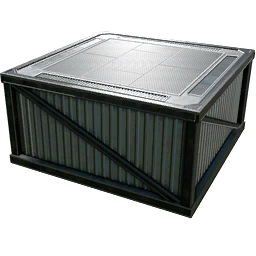
\includegraphics[width=0.07\linewidth]{pictures/fundation}
    \end{center}
\end{frame}


\begin{frame}
    \frametitle{How does it work}
    \begin{center}
        \frame{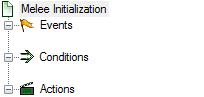
\includegraphics[width=0.6\linewidth]{pictures/event-condition-action.png}}
    \end{center}
    \begin{enumerate}
        \item An \textbf{event} happens in MISP
        \item Check if all \textbf{conditions} are satisfied
        \item Execute all \textbf{actions}
    \end{enumerate}
\end{frame}

\begin{frame}
    \frametitle{What kind of events?}
    
\includegraphics[width=60px]{pictures/sc-event.png}
    \vspace*{0.5em}
    \begin{itemize}
        \item New MISP Event
        \item Attribute has been saved
        \item New discussion post
        \item New user created
        \item Query against third-party services
        \item ...
    \end{itemize}
    \vspace*{1em}
    {\Large \faIcon{question-circle}} Supported events in MISP are called \textbf{Triggers}\\
    {\Large \faIcon{question-circle}} A \textbf{Trigger} is associated with \textbf{1-and-only-1 Workflow}
\end{frame}

\begin{frame}
    \frametitle{Triggers currently available}
    Currently 11 triggers can be hooked. 3 being 
\includegraphics[width=36px]{pictures/blocking-workflow.png}.
    \begin{center}
        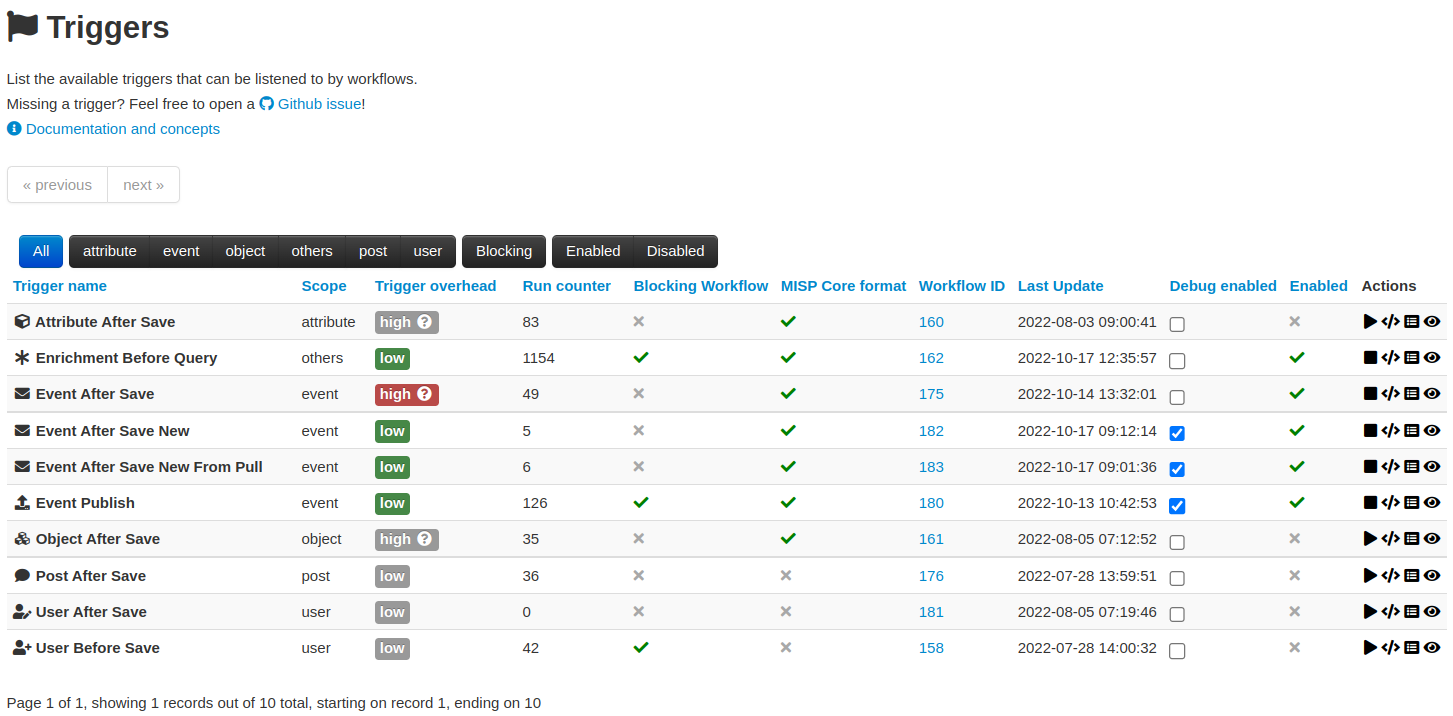
\includegraphics[width=1.0\linewidth]{pictures/triggers.png}
    \end{center}
\end{frame}

\begin{frame}
    \frametitle{What kind of conditions?}
    \vspace*{0.25em}
    
\includegraphics[width=70px]{pictures/sc-condition.png}
    \vspace*{0.25em}
    \begin{itemize}
        \item A MISP Event is tagged with \texttt{tlp:red}
        \item The distribution of an Attribute is a sharing group
        \item The creator organisation is \texttt{circl.lu}
        \item Or any other \textbf{generic} conditions
    \end{itemize}

    \vspace*{0.5em}
    {\Large \faIcon{question-circle}} These are also called \textbf{Logic modules}
    \begin{center}
        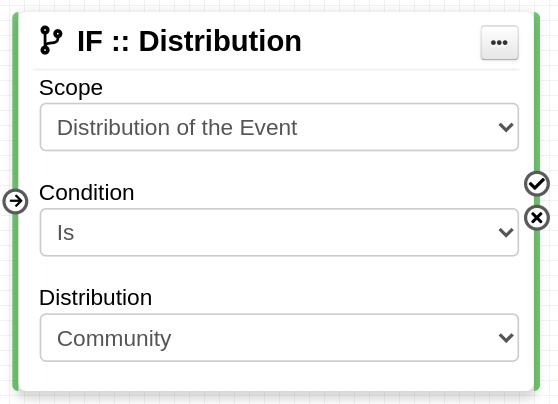
\includegraphics[width=0.43\textwidth]{pictures/logic-module.png}
    \end{center}
\end{frame}

\begin{frame}
    \frametitle{Workflow - Logic modules}
    \begin{itemize}
        \item 
\includegraphics[width=12px]{pictures/sc-condition-icon.png} \textbf{logic} modules: Allow to redirect the execution flow.
        \begin{itemize}
            \item IF conditions
            \item Delay execution
        \end{itemize}
    \end{itemize}
    \begin{center}
        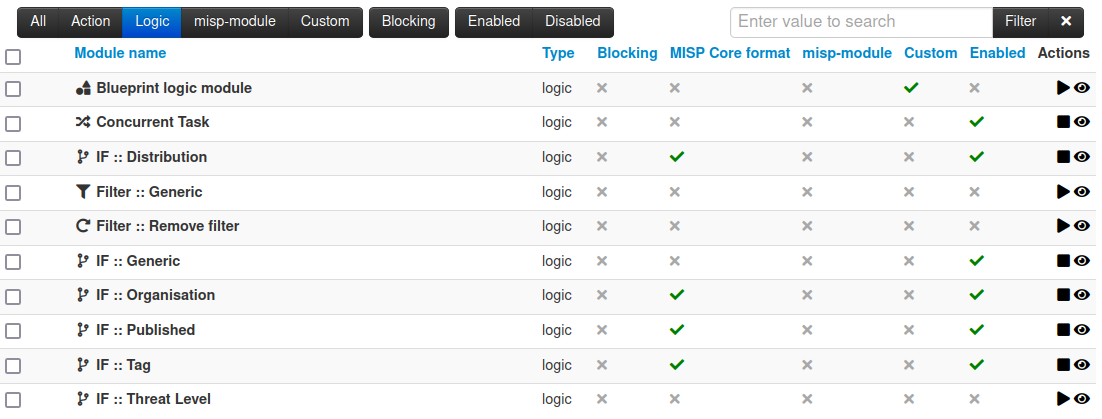
\includegraphics[width=1.0\linewidth]{pictures/logic-module-index.png}
    \end{center}
\end{frame}

\begin{frame}
    \frametitle{What kind of actions?}
    \vspace*{0.25em}
    
\includegraphics[width=60px]{pictures/sc-action.png}
    \vspace*{0.25em}
    \begin{itemize}
        \item Send an email notification
        \item Perform enrichments
        \item Send a chat message on MS Teams
        \item Attach a local tag
        \item ...
    \end{itemize}

    \vspace*{0.5em}
    {\Large \faIcon{question-circle}} These are also called \textbf{Action modules}
    \begin{center}
        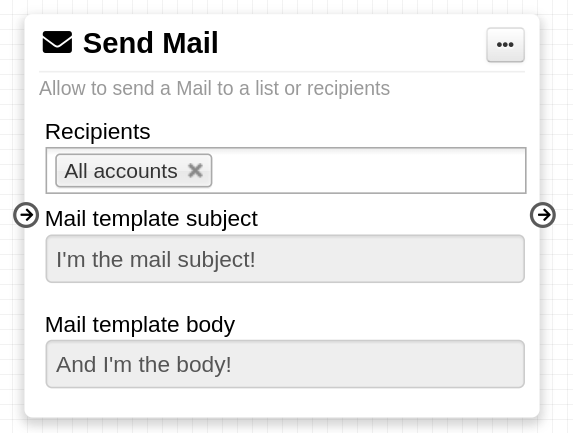
\includegraphics[width=0.43\textwidth]{pictures/action-module.png}
    \end{center}
\end{frame}

\begin{frame}
    \frametitle{Workflow - Action modules}
    \begin{itemize}
        \item 
\includegraphics[width=12px]{pictures/sc-action-icon.png} \textbf{action} modules: Allow to executes operations
        \begin{itemize}
            \item Tag operations
            \item Send notifications
            \item Webhooks \& Custom scripts
        \end{itemize}
    \end{itemize}
    \begin{center}
        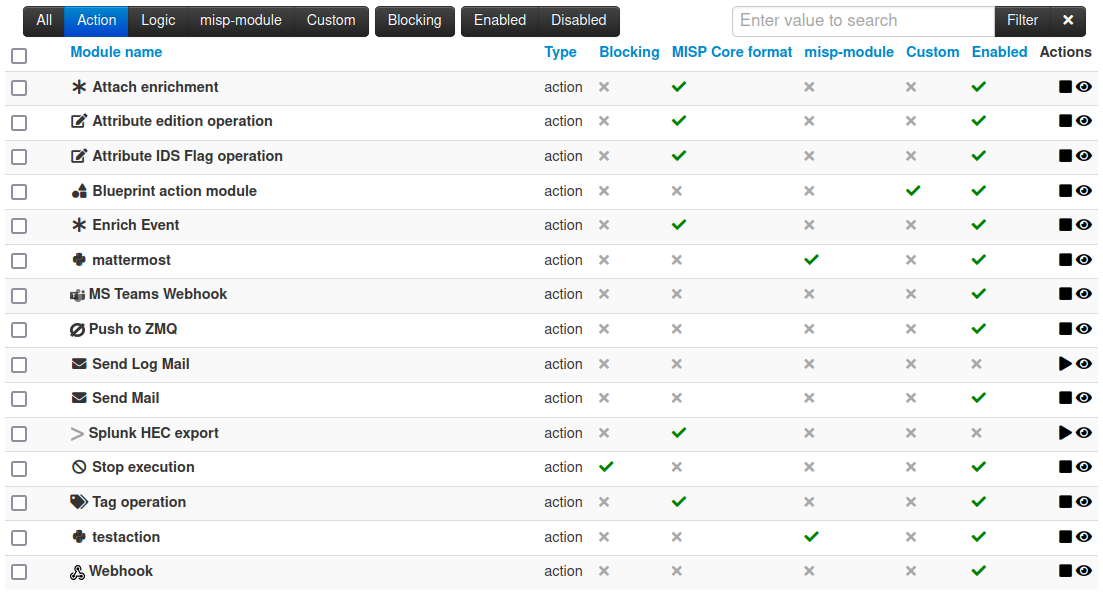
\includegraphics[width=0.95\linewidth]{pictures/action-module-index.png}
    \end{center}
\end{frame}

\begin{frame}
    \frametitle{What is a MISP Workflow?}
    \begin{itemize}
        \item Sequence of all nodes to be executed in a specific order
    \end{itemize}
    \vspace*{0.5em}
    \begin{center}
        \frame{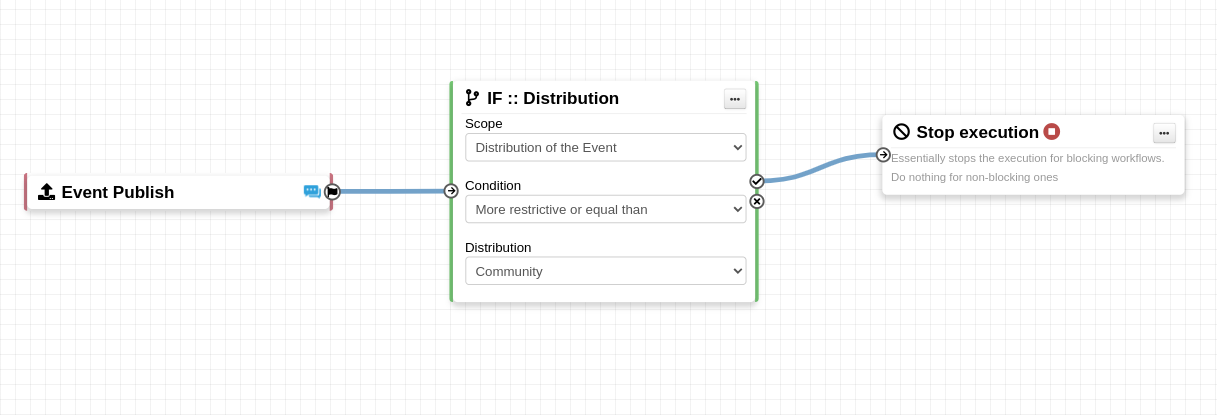
\includegraphics[width=1.0\linewidth]{pictures/simple-workflow.png}}
    \end{center}
\end{frame}

\begin{frame}
    \frametitle{Workflow execution for Event publish}
    \begin{itemize}
        \setlength\itemsep{1em}
        \item[] \hspace*{-2em}
\includegraphics[width=16px]{pictures/sc-event-icon.png} \hspace*{0.25em} An Event is about to be published
        \begin{itemize}
            \item The workflow for the \texttt{event-publish} trigger starts
        \end{itemize}
        \item[] \hspace*{-2em}
\includegraphics[width=16px]{pictures/sc-condition-icon.png} \hspace*{0.25em} Conditions are evaluated
        \begin{itemize}
            \item They might change the path taken during the execution
        \end{itemize}
        \item[] \hspace*{-2em}
\includegraphics[width=16px]{pictures/sc-action-icon.png} \hspace*{0.25em} Actions are executed
        \begin{itemize}
            \setlength\itemsep{0.75em}
            \item {\bf\color{green!50!black}success}: Continue the publishing action
            \hspace*{-4em}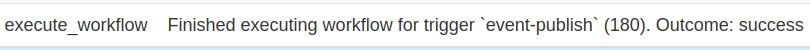
\includegraphics[width=1.0\textwidth]{pictures/log-entry-publish-success.png}
            \item {\bf\color{red}failure} | \texttt{\color{red}blocked}: Stop publishing and log the reason
            \hspace*{-4em}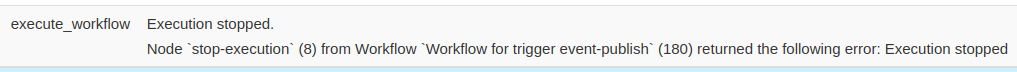
\includegraphics[width=1.0\textwidth]{pictures/log-entry-publish-blocked.png}
        \end{itemize}
    \end{itemize}
\end{frame}


\begin{frame}
    \frametitle{Sources of Workflow modules (0)}
    Currently 36 built-in modules.
    \vspace{1em}
    \begin{itemize}
        \item \textbf{Trigger} module (11): built-in \textbf{only}
        \begin{itemize}
            \item Get in touch if you want more
        \end{itemize}
        \item \textbf{Logic} module (10): built-in \& \textbf{custom}
        \item \textbf{Action} module (15): built-in \& \textbf{custom}
    \end{itemize}
    \vspace*{2.0em}
\end{frame}

\begin{frame}
    \frametitle{Sources of Workflow modules (1)}
    \begin{itemize}
        \item Built-in \textbf{default} modules
        \begin{itemize}
            \item Part of the MISP codebase
            \item Get in touch if you want us to increase the selection (or merge PR!)
        \end{itemize}
    \end{itemize}
    \vspace*{0.5em}
    \begin{center}
        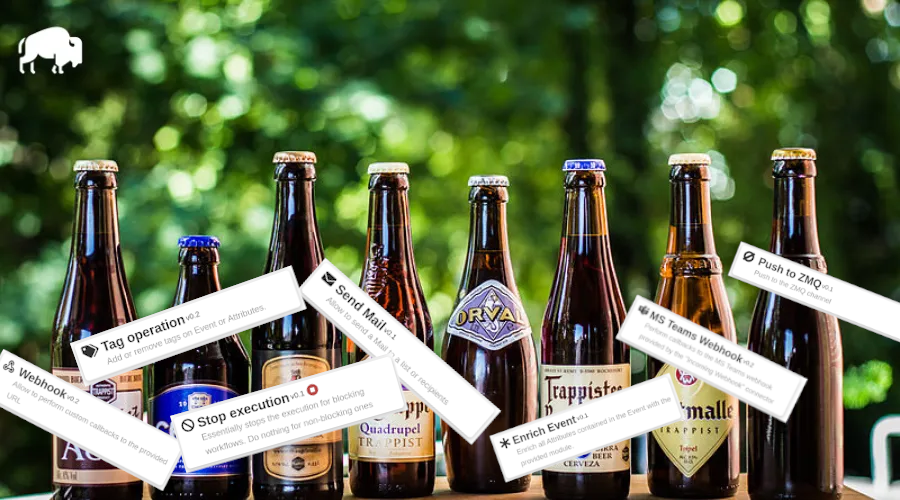
\includegraphics[width=0.8\linewidth]{pictures/module-buffet.png}
    \end{center}
\end{frame}

\begin{frame}
    \frametitle{Sources of Workflow modules (2)}
    User-defined \textbf{custom} modules
    \vspace*{0.5em}
    \begin{columns}
        \begin{column}{0.5\textwidth}
            \begin{itemize}
                \item Written in PHP
                \item Extend existing modules
                \item MISP code reuse
            \end{itemize}
        \end{column}
        \begin{column}{0.5\textwidth}
            
\includegraphics[width=1.0\linewidth]{pictures/php-joke.jpg}
        \end{column}
    \end{columns}
\end{frame}

\begin{frame}
    \frametitle{Sources of Workflow modules (3)}
    Modules from the 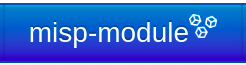
\includegraphics[width=0.20\linewidth]{pictures/misp-module-icon.png} \textbf{enrichment service}
    \vspace*{0.5em}
    \begin{columns}
        \begin{column}{0.50\textwidth}
            \begin{itemize}
                \item Written in Python
                \item Can use any python libraries
                \item Plug \& Play
            \end{itemize}
        \end{column}
        \begin{column}{0.50\textwidth}
            
\includegraphics[width=1.0\linewidth]{pictures/python-joke.png}
        \end{column}
    \end{columns}
\end{frame}

\begin{frame}
    \frametitle{Getting started with workflows (5)}
    \centering
    \vspace*{3em}
    {\LARGE Let's build a workflow!}
    \begin{center}
        
\includegraphics[width=24px]{pictures/build-icon.png}
    \end{center}
\end{frame}

\begin{frame}
    \frametitle{Creating a workflow with the editor}
    \begin{enumerate}
        \item Prevent event publication if \textbf{tlp:red} tag
        \item Send a mail to \texttt{admin@admin.test} about potential data leak
        \item Otherwise, send a notification on \textbf{Mattermost}, \textbf{MS Teams}, \textbf{Telegram}, ...
    \end{enumerate}
\end{frame}

% \section{Considerations when working with workflows}
\begin{frame}
    \frametitle{
        \huge
        \linebreak
        \linebreak
        \linebreak
        Considerations when working with workflows
        \vspace{1em}
    }
    \textbf{Objective:} Overview of some common pitfalls
    \begin{center}
        
\includegraphics[width=24px]{pictures/radar.png}
    \end{center}
\end{frame}

\begin{frame}
    \frametitle{Working with the editor - Operations not allowed}
    Execution loop are not authorized
    \vspace*{1em}
    \begin{columns}
        \begin{column}{0.7\textwidth}
            \frame{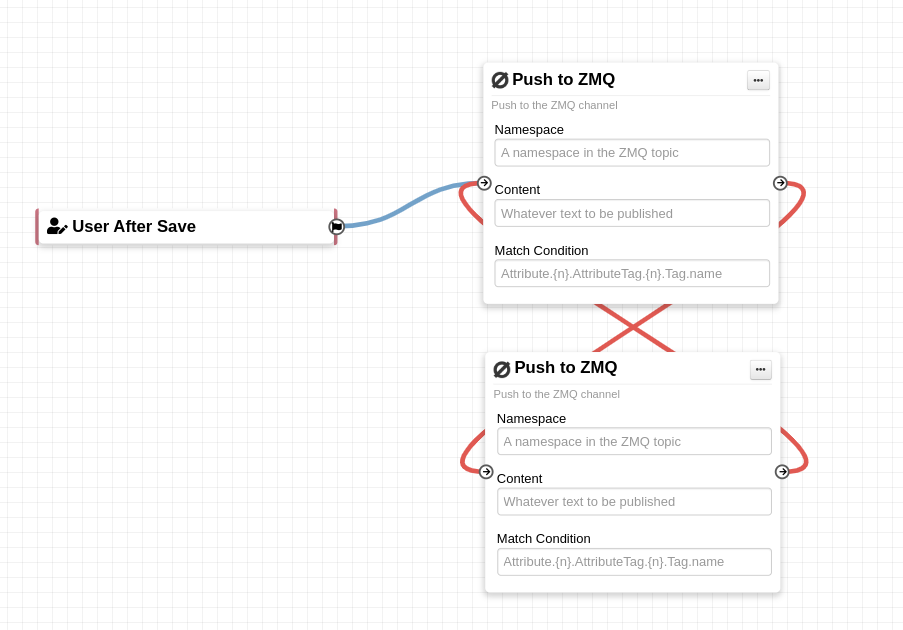
\includegraphics[width=1.0\linewidth]{pictures/editor-not-allowed-1.png}}
        \end{column}
        \begin{column}{0.3\textwidth}
            \frame{
\includegraphics[width=1.0\linewidth]{pictures/infinite-loop.jpg}}
        \end{column}
    \end{columns}
\end{frame}

\begin{frame}
    \frametitle{Recursive workflows}
    \frame{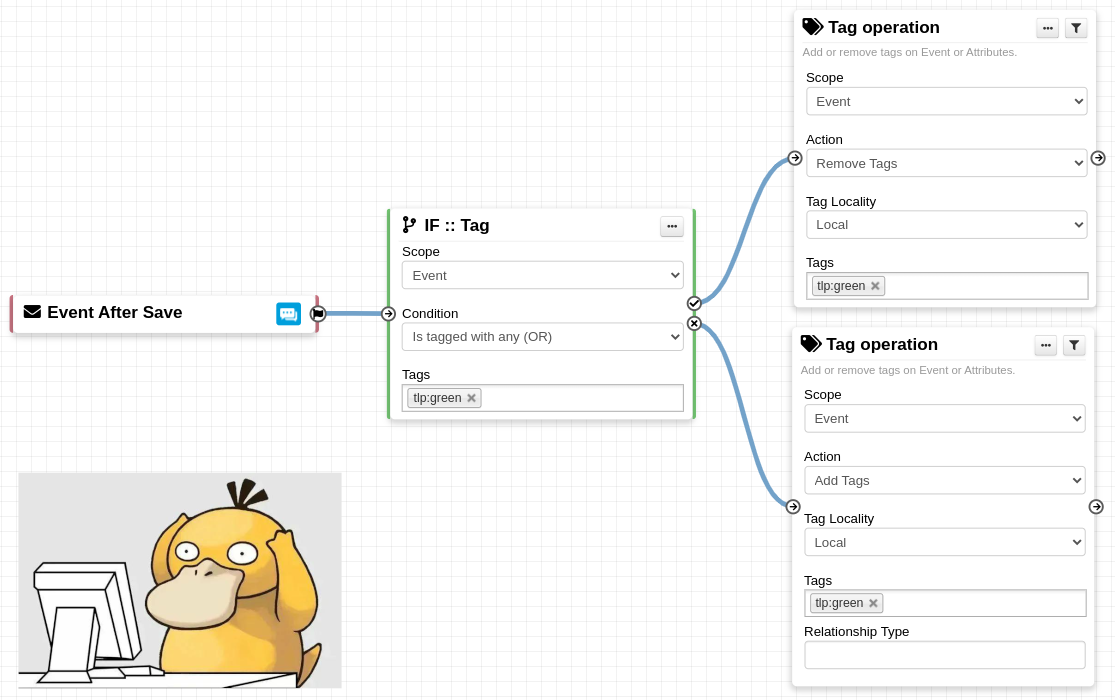
\includegraphics[width=1.0\linewidth]{pictures/recursive-workflow.png}}
    \danger Recursion: If an action re-run the workflow
\end{frame}

\begin{frame}
    \frametitle{Workflow blueprints}
    \hspace*{0.9\textwidth}
\includegraphics[width=32px]{pictures/blueprint-32.png}
    \vspace*{-2em}
    \begin{enumerate}
        \item Blueprints allow to \textbf{re-use parts} of a workflow in another one
        \item Blueprints can be saved, exported and \textbf{shared}
    \end{enumerate}
    \begin{center}
        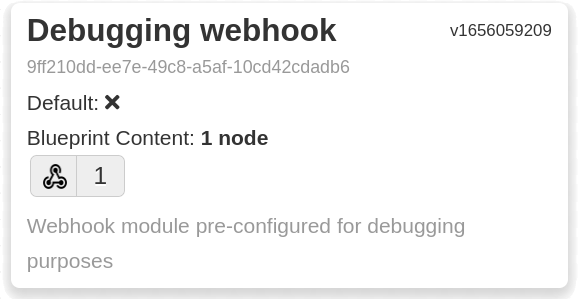
\includegraphics[width=0.5\linewidth]{pictures/blueprint-debugging.png}
    \end{center}
    Blueprints sources:
    \begin{enumerate}
        \item Created or imported by users
        \item From the \texttt{MISP/misp-workflow-blueprints} repository\footnote{\scriptsize https://github.com/MISP/misp-workflow-blueprints}
    \end{enumerate}
\end{frame}

\begin{frame}
    \frametitle{Workflow blueprints}
    Currently, 4 blueprints available:
    \vspace*{1em}
    \begin{itemize}
        \item Attach the \texttt{tlp:clear} tag on elements having the \texttt{tlp:white} tag
        \item Block actions if any attributes have the \texttt{PAP:RED} or \texttt{tlp:red} tag
        \item Disable \texttt{to\_ids} flag for existing hash in \textit{hashlookup}
        \item Set tag based on \textit{BGP Ranking} maliciousness level
    \end{itemize}
\end{frame}

\begin{frame}
    \frametitle{Future works}
    \begin{columns}
        \begin{column}{0.55\textwidth}
            \begin{itemize}
                \item More 
\includegraphics[width=12px]{pictures/sc-action-icon.png} modules
                \item More 
\includegraphics[width=12px]{pictures/sc-condition-icon.png} modules
                \item More 
\includegraphics[width=12px]{pictures/sc-event-icon.png} triggers
                \item More documentation
                \item Recursion prevention system
                \item On-the-fly data override?
            \end{itemize}
        \end{column}
        \begin{column}{0.45\textwidth}
            
\includegraphics[width=1.0\linewidth]{pictures/future-works.jpeg}
        \end{column}
    \end{columns}
\end{frame}

\begin{frame}
    \frametitle{Final words}
    \begin{columns}
        \begin{column}{0.6\textwidth}
            \begin{itemize}
                \item Designed to \textbf{quickly} and \textbf{cheaply} integrate MISP in CTI pipelines
                \item \underline{\textbf{Beta}} Feature unlikely to change. But still..
                \item Waiting for feedback!
                \begin{itemize}
                    \item New triggers?
                    \item New modules?
                    \item What's acheivable
                \end{itemize}
            \end{itemize}
        \end{column}
        \begin{column}{0.4\textwidth}
            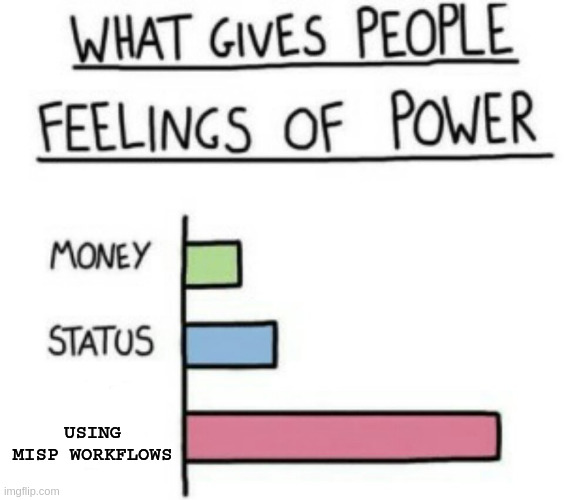
\includegraphics[width=1.0\linewidth]{pictures/feeling-of-power.jpg}
        \end{column}
    \end{columns}
    \vspace*{0.5em}
\end{frame}

